
\documentclass[11pt,a4paper,UTF8]{book}

\usepackage{minted}
\usepackage[T1]{fontenc}
\usepackage[utf8]{inputenc}
\usepackage{authblk}

\usepackage{fontspec}                  %引入字体设置宏包
\setmainfont{Times New Roman}             %设置英文正文字体
% Courier New
% Book Antique
\setsansfont{Arial}                    %英文无衬线字体
\setmonofont{Courier New}              %英文等宽字体

\usepackage{ctex} %导入中文包
%\usepackage{ulem}
\usepackage{tocvsec2}
\usepackage{verbatim}

\usepackage{tabularx}
\usepackage{longtable}
\usepackage{booktabs}
\usepackage{multirow}
\usepackage{bbding}
\usepackage{float}
\usepackage{xspace}
\usepackage[none]{hyphenat}

\usepackage{graphicx}
\usepackage{subfigure}
\usepackage{pifont}

\usepackage{hyperref}  %制作pdf的目录
\usepackage{subfiles} %使用多文件方式进行

\usepackage{geometry} %设置页边距的包
\geometry{left=2.5cm,right=2cm,top=2.54cm,bottom=2.54cm} %设置书籍的页边距

\usepackage{url}
\hypersetup{hidelinks, %去红框
  colorlinks=true,
  allcolors=black,
  pdfstartview=Fit,
  breaklinks=true
}

% 调整itemlist中的行间距
\usepackage{enumitem}
\setenumerate[1]{itemsep=0pt,partopsep=0pt,parsep=\parskip,topsep=5pt}
\setitemize[1]{itemsep=0pt,partopsep=0pt,parsep=\parskip,topsep=5pt}
\setdescription{itemsep=0pt,partopsep=0pt,parsep=\parskip,topsep=5pt}

% 超链接样式设置
\usepackage{hyperref}
\hypersetup{
  colorlinks=true,
  linkcolor=blue,
  filecolor=blue,
  urlcolor=blue,
  citecolor=cyan,
}

\usepackage{indentfirst}

\usepackage{listings}
\usepackage[usenames,dvipsnames,svgnames, x11names]{xcolor}

\usepackage[most]{tcolorbox}
\tcbuselibrary{breakable} % 引入 breakable 库
\tcbuselibrary{skins} % 引入 skins 库

%定义CMake
\lstdefinelanguage{CMake}
{morekeywords={
    cmake\_minimum\_required,
    project,
    add\_executable,
    add\_library,
    target\_link\_libraries,
    cmake\_parse\_arguments,
    cmake\_language,
    set, unset,
    option,
    string,
    list,
    math,
    message,
    if, elseif, else, endif,
    mark\_as\_advanced,
    foreach, endforeach,
    while, endwhile,
    add\_subdirectory, include, return, include\_gurad,
    function, endfunction,
    macro, endmacro,
    find\_package,
    cmake\_push\_check\_state,
    cmake\_pop\_check\_state,
    cmake\_reset\_check\_state,
    add\_test,
    set\_tests\_properties,
    check\_c\_source\_runs,
    check\_cxx\_source\_runs,
    check\_fortran\_source\_runs,
    check\_source\_runs,
    check\_compiler\_flag,
    check\_c\_compiler\_flag,
    check\_cxx\_compiler\_flag,
    check\_fortran\_compiler\_flag,
    check\_symbol\_exists,
    check\_cxx\_symbol\_exists,
    check\_linker\_flag,
    cmake\_policy,
    set\_property,
    get\_property,
    define\_property,
    get\_cmake\_property,
    set\_cmake\_property,
    set\_target\_properties,
    get\_target\_property,
    set\_directory\_properties,
    get\_directory\_property,
    set\_source\_files\_properties,
    get\_source\_file\_property,
    set\_tests\_properties,
    get\_tests\_property,
    get\_test\_property,
    cmake\_print\_properties,
    cmake\_print\_variables,
    variable\_watch,
    include\_guard,
    target\_link\_options,
    target\_compile\_definitions,
    target\_compile\_options,
    include\_directories,
    add\_definitions,
    remove\_definitions,
    add\_compile\_definitions,
    add\_compile\_options,
    link\_libraries,
    link\_directories,
    add\_link\_options,
    target\_include\_directories,
    target\_compile\_features,
    add\_custom\_command,
    add\_custom\_target,
    execute\_process,
    cmake\_path,
    get\_filename\_component,
    file,
    configure\_file,
    generate\_export\_header,
    export,
    find\_file,
    find\_library,
    find\_package,
    find\_program,
    pkg\_check\_modules,
    pkg\_search\_module,
    pkg\_get\_variable,
    add\_test,
    enable\_testing,
    set\_tests\_properties,
    site\_name,
    ctest\_empty\_binary\_directory,
    ctest\_start,
    ctest\_configure,
    ctest\_submit,
    ctest\_build,
    ctest\_memcheck,
    ctest\_upload,
    ctest\_test,
    gtest\_add\_tests,
    gtest\_discover\_tests,
    install,
    write\_basic\_package\_version\_file,
    configure\_package\_config\_file,
    cpack\_add\_component,
    cpack\_add\_install\_type,
    cpack\_add\_component\_group,
    ExternalProject\_Add,
    ExternalProject\_Add\_StepDependencies,
    ExternalProject\_Get\_Property,
    ExternalProject\_Add\_Step,
    FetchContent\_Declare,
    FetchContent\_GetProperties,
    FetchContent\_Populate,
    source\_group,
    target\_precompile\_headers,
    qt5\_wrap\_cpp,
    qt5\_wrap\_ui,
    qt5\_add\_resources,
    qt5\_add\_big\_resources,
    qt5\_add\_binary\_resources,
    qt5\_add\_translation,
    qt5\_create\_translation,
    compile\_definitions,
    add\_llvm\_component\_library,
    add\_llvm\_tool,
    llvm\_multisource,
    llvm\_test\_data,
    doxygen\_add\_docs,
    cmake\_dependent\_option,
    target\_sources,
    conan\_cmake\_autodetect,
    conan\_cmake\_configure,
    conan\_cmake\_install,
    doxygen\_add\_docs,
    check\_source\_compiles,
    check\_language,
    enable\_language,
    add\_dependencies,
    find\_path,
    find\_package\_handle\_standard\_args,
  }, %定义关键字
  sensitive=false, %是否大小写敏感
  morecomment=[l]{\#},
  morestring=[b]",
  morestring=[d]',
}

\lstdefinestyle{styleCMake}{
  language=CMake,
  backgroundcolor=\color{blue!3!white},
  basicstyle=\tt,
  breakatwhitespace = false,
  breaklines = true,
  captionpos = b,
  commentstyle = \color{mygray}\bfseries,
  extendedchars =false,
  frame=shadowbox,
  tabsize=2,
  framerule=0.5pt,
  keepspaces=true,
  keywordstyle=\color{blue}\bfseries, % keyword style
  otherkeywords={string},
  rulecolor=\color{black},
  showspaces=false,
  showstringspaces=false,
  showtabs=false,
  stepnumber=1,
  stringstyle=\color{purple},        % string literal style
}

\lstdefinestyle{stylePython}{
  language        =   Python, % 语言选Python
  backgroundcolor=\color{blue!3!white},
  basicstyle      =   \zihao{-5}\ttfamily,
  numberstyle     =   \zihao{-5}\ttfamily,
  keywordstyle    =   \color{blue},
  keywordstyle    =   [2] \color{teal},
  stringstyle     =   \color{magenta},
  commentstyle    =   \color{red}\ttfamily,
  frame = shadowbox,
  breaklines      =   true,   % 自动换行,建议不要写太长的行
  columns         =   fixed,  % 如果不加这一句,字间距就不固定,很丑,必须加
  basewidth       =   0.5em,
  %basicstyle          =   \sffamily,          % 基本代码风格
  %keywordstyle        =   \bfseries,          % 关键字风格
  %commentstyle        =   \rmfamily\itshape,  % 注释的风格,斜体
  %stringstyle         =   \ttfamily,  % 字符串风格
  flexiblecolumns,                % 别问为什么,加上这个
  %numbers             =   left,   % 行号的位置在左边
  showspaces          =   false,  % 是否显示空格,显示了有点乱,所以不现实了
  numberstyle         =   \zihao{-5}\ttfamily,    % 行号的样式,小五号,tt等宽字体
  showstringspaces    =   false,
  captionpos          =   t,      % 这段代码的名字所呈现的位置,t指的是top上面
  frame               =   lrtb,   % 显示边框
  tabsize=2,
}

\tcbset{
  breakable,
  commandshell/.style={
    listing only,
    colback=black!75!white,
    colupper=white,
    lowerbox=ignored,
    listing options={
      language={bash},
      breaklines=true,
      basicstyle=\ttfamily,
      columns = fixed,
      flexiblecolumns
    }
}}

\usepackage{tikz}

% URL 正确换行
% https://liam.page/2017/05/17/help-the-url-command-from-hyperref-to-break-at-line-wrapping-point/
\makeatletter
\def\UrlAlphabet{%
  \do\a\do\b\do\c\do\d\do\e\do\f\do\g\do\h\do\i\do\j%
  \do\k\do\l\do\m\do\n\do\o\do\p\do\q\do\r\do\s\do\t%
  \do\u\do\v\do\w\do\x\do\y\do\z\do\A\do\B\do\C\do\D%
  \do\E\do\F\do\G\do\H\do\I\do\J\do\K\do\L\do\M\do\N%
  \do\O\do\P\do\Q\do\R\do\S\do\T\do\U\do\V\do\W\do\X%
  \do\Y\do\Z}
\def\UrlDigits{\do\1\do\2\do\3\do\4\do\5\do\6\do\7\do\8\do\9\do\0}
\g@addto@macro{\UrlBreaks}{\UrlOrds}
\g@addto@macro{\UrlBreaks}{\UrlAlphabet}
\g@addto@macro{\UrlBreaks}{\UrlDigits}
\makeatother

% enable subsubsubsection
% from https://tex.stackexchange.com/练习题/274212/correct-hierarchy-levels-of-pdf-bookmarks-for-custom-section-subsubsubsection
\usepackage[depth=3]{bookmark}
\setcounter{secnumdepth}{3}
\setcounter{tocdepth}{4}
\hypersetup{bookmarksdepth=4}

\makeatletter

\newcommand{\toclevel@subsubsubsection}{4}
\newcounter{subsubsubsection}[subsubsection]

\renewcommand{\thesubsubsubsection}{\thesubsubsection.\arabic{subsubsubsection}}

\newcommand{\subsubsubsection}{\@startsection{subsubsubsection}{4}{\z@}%
  {-3.25ex\@plus -1ex \@minus -.2ex}%
  {1.5ex \@plus .2ex}%
  {\normalfont\normalsize\bf\bfseries}}

\newcommand*{\l@subsubsubsection}{\@dottedtocline{4}{11em}{5em}}

\newcommand{\subsubsubsectionmark}[1]{}
\makeatother

\ExplSyntaxOn

% Setup enumerate, itemize and description
\setenumerate  { nosep }
\setitemize    { nosep }
\setdescription{ nosep }

% Setup minted
\setminted { obeytabs, tabsize=2, breaklines=true, fontsize=\footnotesize, frame=single }

% Def \filename
\NewDocumentCommand { \filename } { m }
{ \noindent  \hspace*{\fill} \\ \textit { #1 } \vspace*{ -1ex } \nopagebreak[4] }

% Def \mySamllsection
\NewDocumentCommand { \mySamllsection } { m }
{ \noindent \hspace*{\fill} \\ \textbf { #1 } \vspace*{ -1ex } \nopagebreak[4] \\ }

\NewDocumentCommand { \myGraphic } { mmm }
{
  \begin{center}
    \includegraphics[width={#1}\textwidth]{#2}\\
    {#3}
  \end{center}
}

% Def \inlcpp
\NewDocumentCommand { \inlcpp }   { m }
{ \mintinline { cpp } { #1 } }

% Def cpp environment
\NewDocumentEnvironment { cpp } { }
{ \VerbatimEnvironment
  \begin { minted } [ linenos=true ] { cpp } }
{ \end   { minted } }

% Def shell environment
\NewDocumentEnvironment { shell } { }
{ \VerbatimEnvironment
  \begin { minted } { text } }
{ \end   { minted } }

\NewDocumentEnvironment { myNotic } { m }
{ \hspace*{\fill} \\
  \begin { tcolorbox } [ breakable,colback = blue!5!white, colframe=blue!55!black ,title={#1}] }
{ \end   { tcolorbox } }

\NewDocumentEnvironment { myTip } { m }
{ \hspace*{\fill} \\
  \begin { tcolorbox } [ breakable,colback = green!5!white, colframe=green!45!black ,title={#1}] }
{ \end   { tcolorbox } }

\NewDocumentEnvironment { myWarning } { m }
{ \hspace*{\fill} \\
  \begin { tcolorbox } [ breakable,colback=red!5!white,colframe=red!55!black,title={#1}] }
{ \end   { tcolorbox } }

\NewDocumentCommand { \mySubsubsection } { mm }
{
\subsubsection*{\zihao{3} {#1} \hspace{0.2cm}{#2}}
\addcontentsline{toc}{subsubsection}{{#1}\hspace{0.2cm}{#2}}
}

\NewDocumentCommand { \mySubsection } { mmm }
{
\subsection*{\zihao{3}{#1}\hspace{0.2cm}{#2}}
\addcontentsline{toc}{subsection}{{#1}\hspace{0.2cm}{#2}}
\subfile{{#3}}
}

\NewDocumentCommand { \mySection } { mmm }
{
\section*{\zihao{2}{#1}\hspace{0.5cm}{#2}}
\addcontentsline{toc}{section}{{#1}\hspace{0.5cm}{#2}}
\subfile{{#3}}
}

% Latex如何在文本模式批量处理下划线
% https://zhuanlan.zhihu.com/p/615108006

\ExplSyntaxOff

\begin{document}
  \begin{sloppypar} %latex中一行文字出现溢出问题的解决方法
    %\maketitle

    \begin{center}
      \thispagestyle{empty}
      %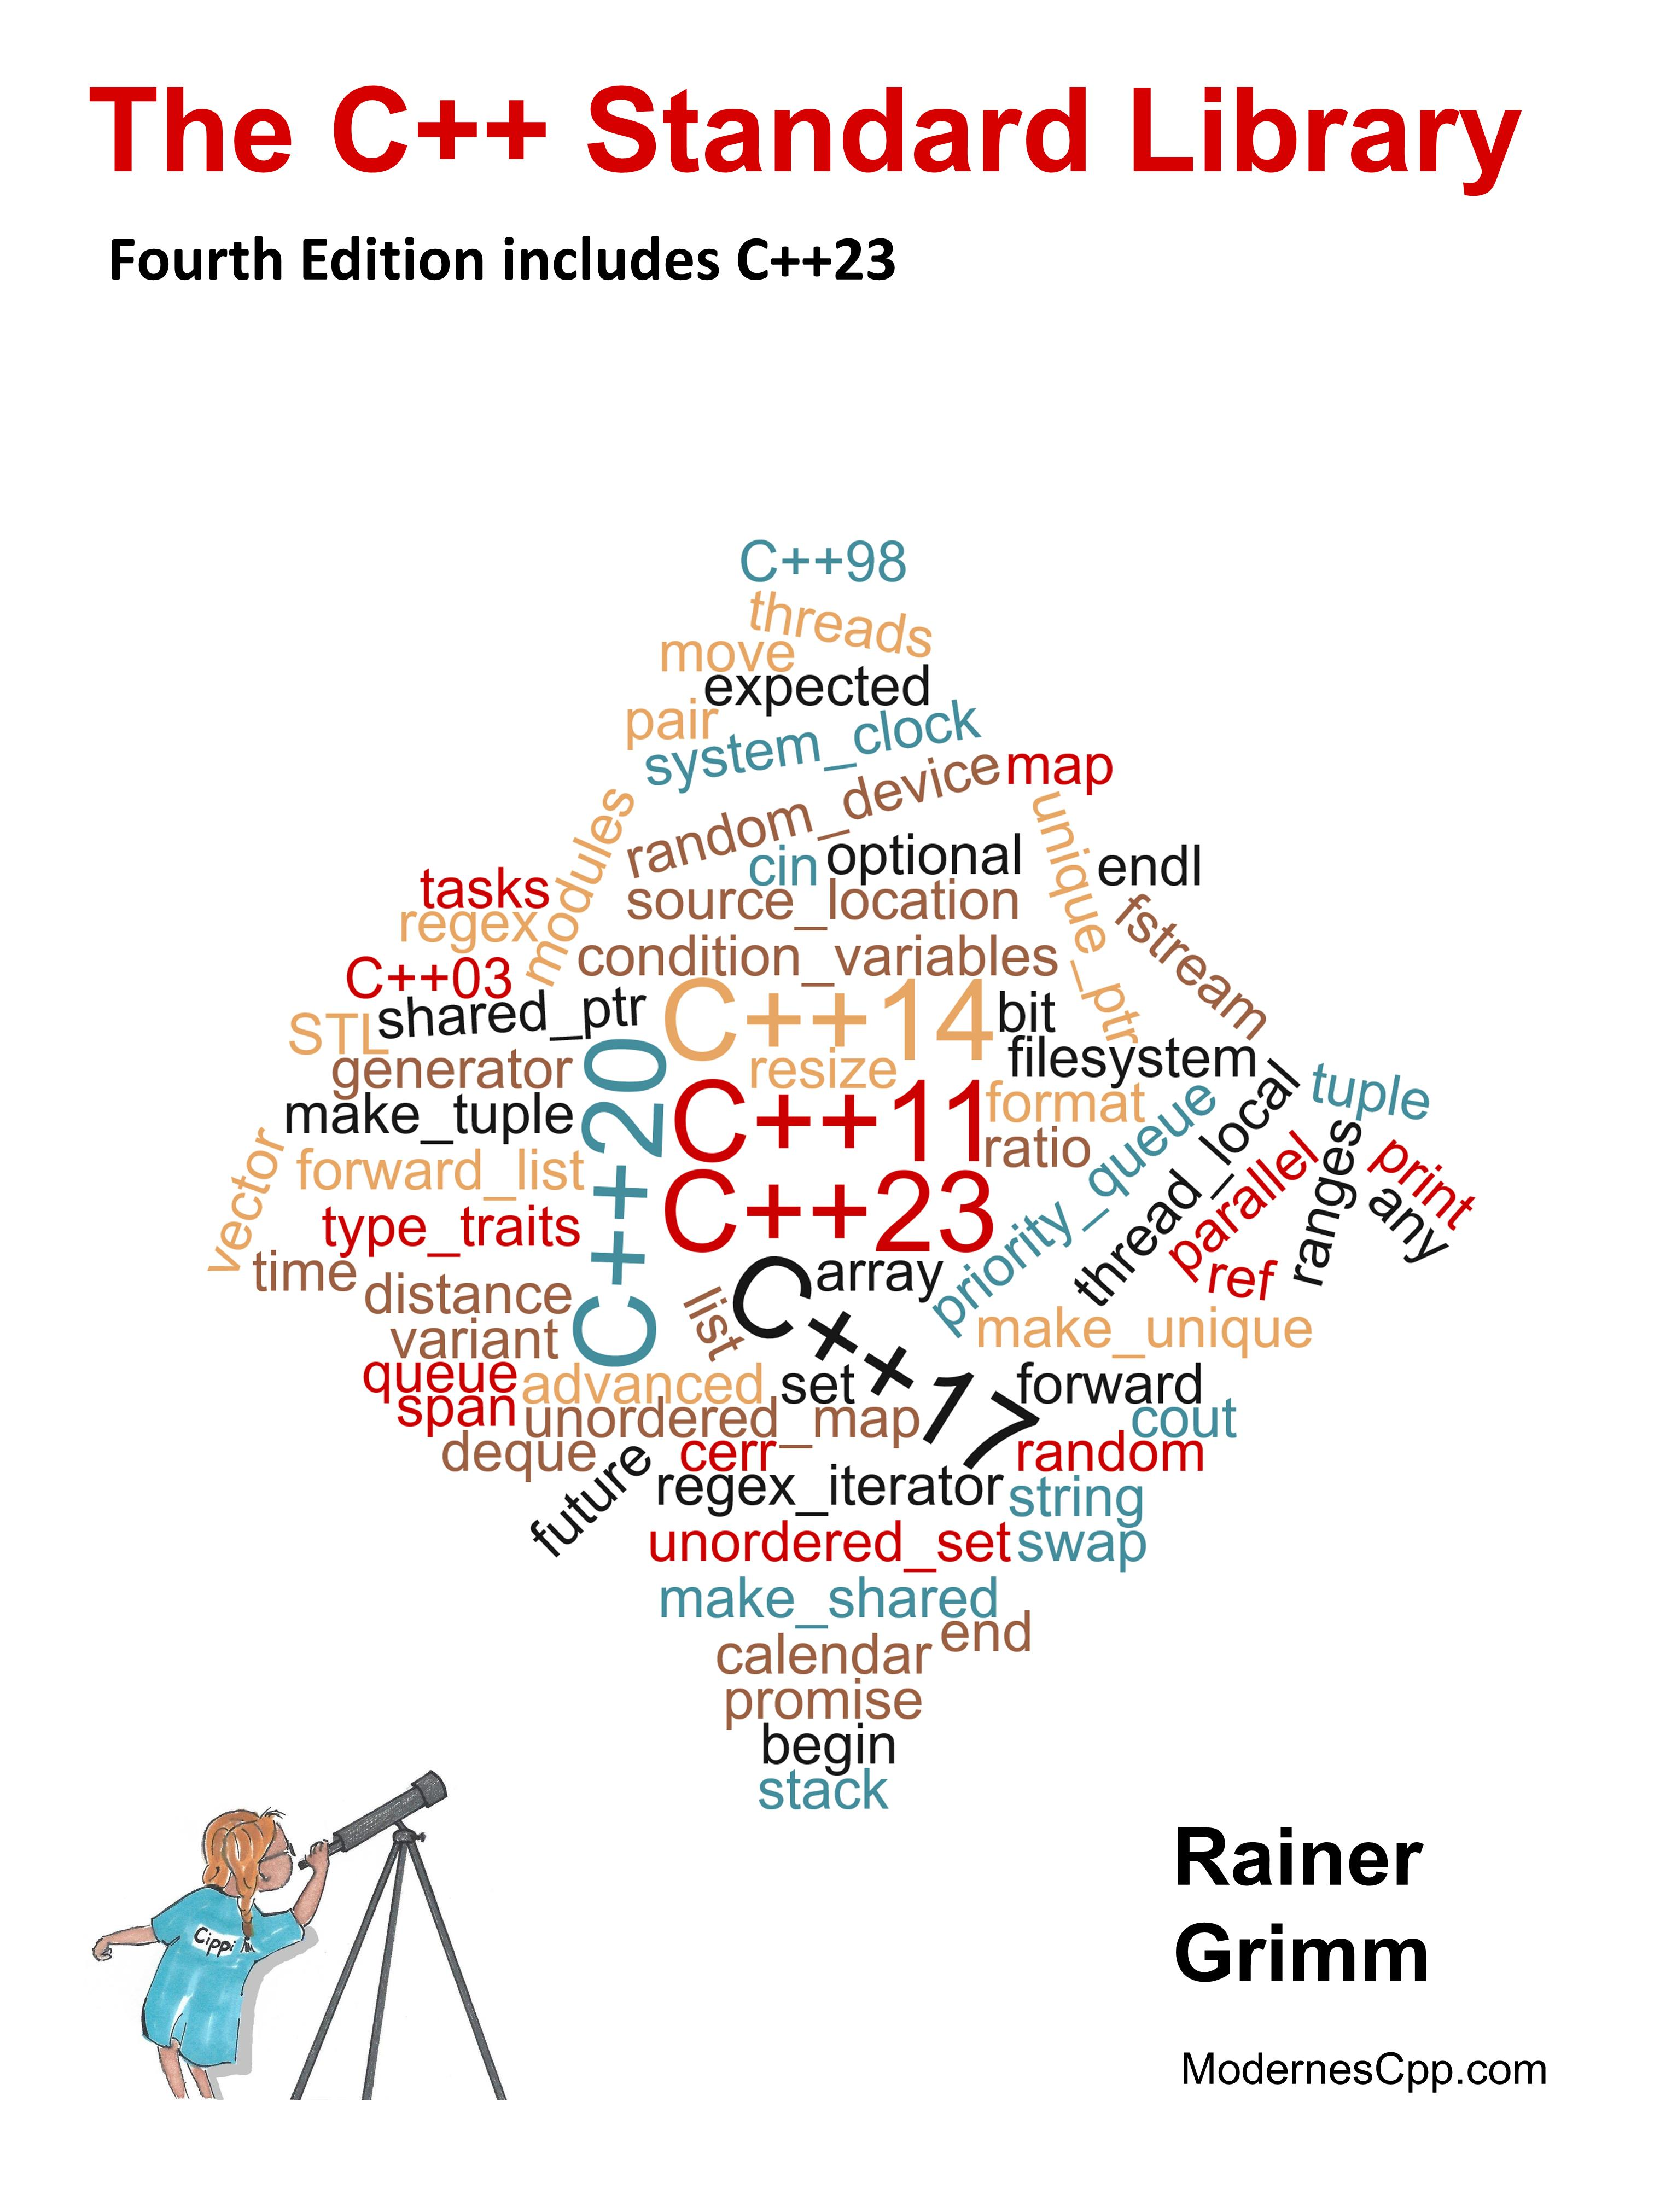
\includegraphics[width=\textwidth,height=\textheight,keepaspectratio]{cover.jpg}
      \begin{tikzpicture}[remember picture, overlay, inner sep=0pt]
        \node at (current page.center)
        {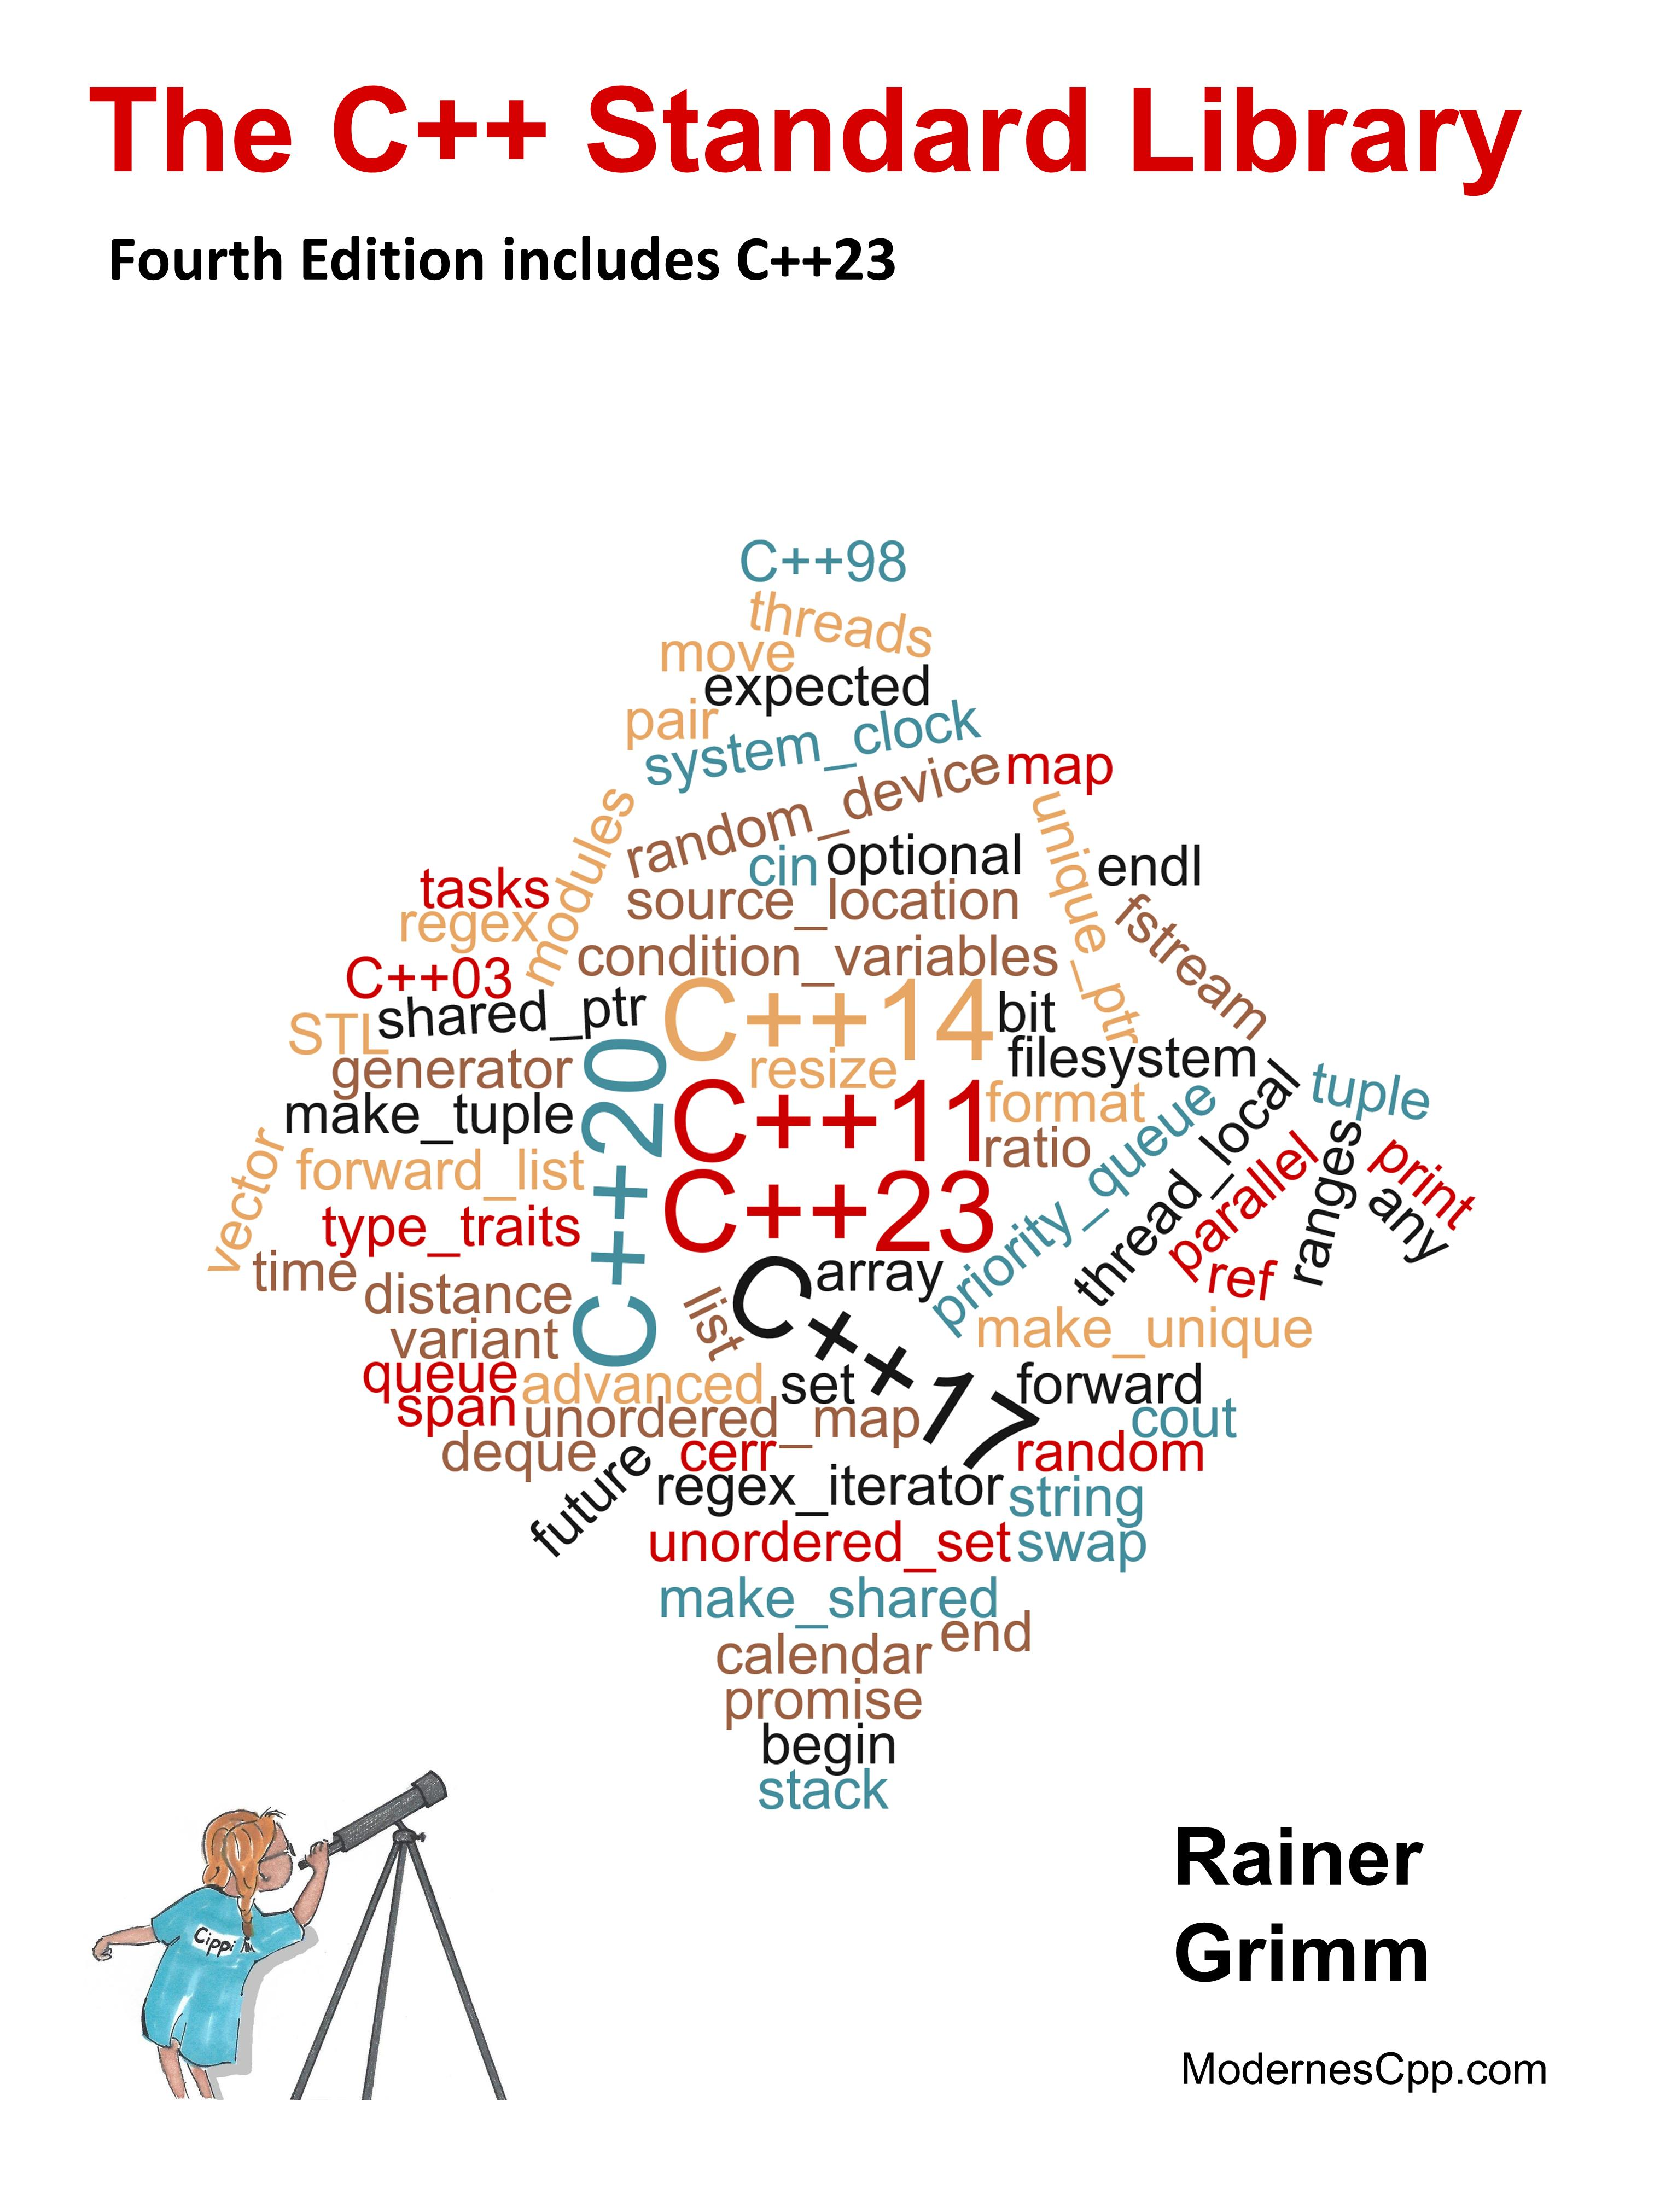
\includegraphics[width=\paperwidth, keepaspectratio=false]{cover.jpg}};
      \end{tikzpicture}
      \newpage
      \thispagestyle{empty}
      \huge
      \textbf{The C++ Standard Library}
      \\[9pt]
      What every professional C++ programmer should know about the C++ standard library.\\[9pt]
      \normalsize
      作者: Rainer Grimm
      \\[8pt]
      \normalsize
      译者:\href{https://github.com/xiaoweiChen/The-CXX-Library-Fourth-EDdition-include-CXX23}{陈晓伟}
      \\[8pt]
      \normalsize
      版本:\href{http://leanpub.com/cpplibrary}{2023-03-11}
    \end{center}

    \newpage

    \pagestyle{empty}
    \tableofcontents
    \newpage

    \setsecnumdepth{section}

    \mySection{}{本书目标}{content/chapter0/0.tex}
    \mySubsection{}{说明}{content/chapter0/1.tex}
    \mySubsection{}{致谢}{content/chapter0/2.tex}
    \mySubsection{}{更多信息}{content/chapter0/3.tex}
    \mySubsection{}{Cippi}{content/chapter0/4.tex}
    \mySubsection{}{关于作者}{content/chapter0/5.tex}
    \newpage

    \mySection{第1章}{标准库}{content/chapter1/0.tex}
    \mySubsection{1.1.}{历史背景}{content/chapter1/1.tex}
    \mySubsection{1.2.}{概述}{content/chapter1/2.tex}
    \mySubsection{1.3.}{如何使用}{content/chapter1/3.tex}
    \newpage

    \mySection{第2章}{实用工具}{content/chapter2/0.tex}
    \mySubsection{2.1.}{有用的功能}{content/chapter2/1.tex}
    \mySubsection{2.2.}{函数适配器}{content/chapter2/2.tex}
    \mySubsection{2.3.}{对子}{content/chapter2/3.tex}
    \mySubsection{2.4.}{元组}{content/chapter2/4.tex}
    \mySubsection{2.5.}{引用包装器}{content/chapter2/5.tex}
    \mySubsection{2.6.}{智能指针}{content/chapter2/6.tex}
    \mySubsection{2.7.}{类型特性}{content/chapter2/7.tex}
    \mySubsection{2.8.}{时间库}{content/chapter2/8.tex}
    \mySubsection{2.9.}{std::any, std::optional和std::variant}{content/chapter2/9.tex}
    \mySubsection{2.10.}{std::expected}{content/chapter2/10.tex}
    \newpage

    \mySection{第3章}{所有容器的接口}{content/chapter3/0.tex}
    \mySubsection{3.1.}{创建和删除}{content/chapter3/1.tex}
    \mySubsection{3.2.}{大小}{content/chapter3/2.tex}
    \mySubsection{3.3.}{访问方式}{content/chapter3/3.tex}
    \mySubsection{3.4.}{赋值和交换}{content/chapter3/4.tex}
    \mySubsection{3.5.}{比较}{content/chapter3/5.tex}
    \mySubsection{3.6.}{擦除}{content/chapter3/6.tex}
    \newpage

    \mySection{第4章}{顺序容器}{content/chapter4/0.tex}
    \mySubsection{4.1.}{Array}{content/chapter4/1.tex}
    \mySubsection{4.2.}{Vector}{content/chapter4/2.tex}
    \mySubsection{4.3.}{Deque}{content/chapter4/3.tex}
    \mySubsection{4.4.}{List}{content/chapter4/4.tex}
    \mySubsection{4.5.}{前向List}{content/chapter4/5.tex}
    \newpage

    \mySection{第5章}{关联容器}{content/chapter5/0.tex}
    \mySubsection{5.1.}{概述}{content/chapter5/1.tex}
    \mySubsection{5.2.}{有序关联容器}{content/chapter5/2.tex}
    \mySubsection{5.3.}{无序关联容器}{content/chapter5/3.tex}
    \newpage

    \mySection{第6章}{容器适配器}{content/chapter6/0.tex}
    \mySubsection{6.1.}{线性容器}{content/chapter6/1.tex}
    \mySubsection{6.2.}{关联性容器}{content/chapter6/2.tex}
    \newpage

    \mySection{第7章}{视图}{content/chapter7/0.tex}
    \mySubsection{7.1.}{连续访问}{content/chapter7/1.tex}
    \mySubsection{7.2.}{多维访问}{content/chapter7/2.tex}
    \newpage

    \mySection{第8章}{迭代器}{content/chapter8/0.tex}
    \mySubsection{8.1.}{类型}{content/chapter8/1.tex}
    \mySubsection{8.2.}{创建迭代器}{content/chapter8/2.tex}
    \mySubsection{8.3.}{实用的功能}{content/chapter8/3.tex}
    \mySubsection{8.4.}{适配器}{content/chapter8/4.tex}
    \newpage

    \mySection{第9章}{可调用单元}{content/chapter9/0.tex}
    \mySubsection{9.1.}{函数}{content/chapter9/1.tex}
    \mySubsection{9.2.}{函数对象}{content/chapter9/2.tex}
    \mySubsection{9.3.}{Lambda函数}{content/chapter9/3.tex}
    \newpage

    \mySection{第10章}{算法}{content/chapter10/0.tex}
    \mySubsection{10.1.}{约定}{content/chapter10/1.tex}
    \mySubsection{10.2.}{迭代器是粘合剂}{content/chapter10/2.tex}
    \mySubsection{10.3.}{顺序,并行或并行执行与先向量化}{content/chapter10/3.tex}
    \mySubsection{10.4.}{for\_each}{content/chapter10/4.tex}
    \mySubsection{10.5.}{不可修改算法}{content/chapter10/5.tex}
    \mySubsection{10.6.}{可修改算法}{content/chapter10/6.tex}
    \mySubsection{10.7.}{分区}{content/chapter10/7.tex}
    \mySubsection{10.8.}{排序}{content/chapter10/8.tex}
    \mySubsection{10.9.}{二分查找}{content/chapter10/9.tex}
    \mySubsection{10.10.}{合并操作}{content/chapter10/10.tex}
    \mySubsection{10.11.}{堆}{content/chapter10/11.tex}
    \mySubsection{10.12.}{最小和最大}{content/chapter10/12.tex}
    \mySubsection{10.13.}{排列}{content/chapter10/13.tex}
    \mySubsection{10.14.}{数值}{content/chapter10/14.tex}
    \mySubsection{10.15.}{单元化内存}{content/chapter10/15.tex}
    \newpage

    \mySection{第11章}{范围库}{content/chapter11/0.tex}
    \mySubsection{11.1.}{范围}{content/chapter11/1.tex}
    \mySubsection{11.2.}{视图}{content/chapter11/2.tex}
    \mySubsection{11.3.}{范围适配器}{content/chapter11/3.tex}
    \mySubsection{11.4.}{直接用于容器}{content/chapter11/4.tex}
    \mySubsection{11.5.}{函数复合}{content/chapter11/5.tex}
    \mySubsection{11.6.}{惰性计算}{content/chapter11/6.tex}
    \mySubsection{11.7.}{std的算法与std::ranges的算法}{content/chapter11/7.tex}
    \newpage

    \mySection{第12章}{数值}{content/chapter12/0.tex}
    \mySubsection{12.1.}{随机数}{content/chapter12/1.tex}
    \mySubsection{12.2.}{从C继承的数值函数}{content/chapter12/2.tex}
    \mySubsection{12.3.}{数学常数}{content/chapter12/3.tex}
    \newpage

    \mySection{第13章}{字符串}{content/chapter13/0.tex}
    \mySubsection{13.1.}{创建和删除}{content/chapter13/1.tex}
    \mySubsection{13.2.}{C++和C字符串之间的转换}{content/chapter13/2.tex}
    \mySubsection{13.3.}{尺寸与容量}{content/chapter13/3.tex}
    \mySubsection{13.4.}{比较}{content/chapter13/4.tex}
    \mySubsection{13.5.}{字符串连接}{content/chapter13/5.tex}
    \mySubsection{13.6.}{访问元素}{content/chapter13/6.tex}
    \mySubsection{13.7.}{输入与输出}{content/chapter13/7.tex}
    \mySubsection{13.8.}{搜索}{content/chapter13/8.tex}
    \mySubsection{13.9.}{检查是否有子字符串}{content/chapter13/9.tex}
    \mySubsection{13.10.}{修改操作}{content/chapter13/10.tex}
    \mySubsection{13.11.}{数值转换}{content/chapter13/11.tex}
    \newpage

    \mySection{第14章}{字符串视图}{content/chapter14/0.tex}
    \mySubsection{14.1.}{创建和初始化}{content/chapter14/1.tex}
    \mySubsection{14.2.}{不可修改的操作}{content/chapter14/2.tex}
    \mySubsection{14.3.}{可修改的操作}{content/chapter14/3.tex}
    \newpage

    \mySection{第15章}{正则表达式}{content/chapter15/0.tex}
    \mySubsection{15.1.}{字符类型}{content/chapter15/1.tex}
    \mySubsection{15.2.}{正则表达式对象}{content/chapter15/2.tex}
    \mySubsection{15.3.}{搜索结果match\_results}{content/chapter15/3.tex}
    \mySubsection{15.4.}{匹配}{content/chapter15/4.tex}
    \mySubsection{15.5.}{搜索}{content/chapter15/5.tex}
    \mySubsection{15.6.}{替换}{content/chapter15/6.tex}
    \mySubsection{15.7.}{格式}{content/chapter15/7.tex}
    \mySubsection{15.8.}{反复搜索}{content/chapter15/8.tex}
    \newpage

    \mySection{第16章}{输入和输出流}{content/chapter16/0.tex}
    \mySubsection{16.1.}{层次结构}{content/chapter16/1.tex}
    \mySubsection{16.2.}{输入输出函数}{content/chapter16/2.tex}
    \mySubsection{16.3.}{流}{content/chapter16/3.tex}
    \mySubsection{16.4.}{自定义数据类型}{content/chapter16/4.tex}
    \newpage

    \mySection{第17章}{格式库}{content/chapter17/0.tex}
    \mySubsection{17.1.}{格式化功能}{content/chapter17/1.tex}
    \mySubsection{17.2.}{语法}{content/chapter17/2.tex}
    \mySubsection{17.3.}{格式规范}{content/chapter17/3.tex}
    \mySubsection{17.4.}{自定义格式化器}{content/chapter17/4.tex}
    \newpage

    \mySection{第18章}{文件系统}{content/chapter18/0.tex}
    \mySubsection{18.1.}{类}{content/chapter18/1.tex}
    \mySubsection{18.2.}{非成员函数}{content/chapter18/2.tex}
    \mySubsection{18.3.}{文件类型}{content/chapter18/3.tex}
    \newpage

    \mySection{第19章}{多线程}{content/chapter19/0.tex}
    \mySubsection{19.1.}{内存模型}{content/chapter19/1.tex}
    \mySubsection{19.2.}{原子数据类型}{content/chapter19/2.tex}
    \mySubsection{19.3.}{线程}{content/chapter19/3.tex}
    \mySubsection{19.4.}{停止令牌}{content/chapter19/4.tex}
    \mySubsection{19.5.}{共享变量}{content/chapter19/5.tex}
    \mySubsection{19.6.}{线程本地数据}{content/chapter19/6.tex}
    \mySubsection{19.7.}{条件变量}{content/chapter19/7.tex}
    \mySubsection{19.8.}{信号量}{content/chapter19/8.tex}
    \mySubsection{19.9.}{协调类型}{content/chapter19/9.tex}
    \mySubsection{19.10.}{任务}{content/chapter19/10.tex}
    \newpage

    \mySection{第20章}{协程}{content/chapter20/0.tex}
    \mySubsection{20.1.}{可等待}{content/chapter20/1.tex}
    \mySubsection{20.2.}{无限数据流——co\_yield}{content/chapter20/2.tex}
    \newpage

  \end{sloppypar}
\end{document}

